\documentclass[tikz,border=5pt]{standalone}
\usepackage{amsmath,amssymb}
\usetikzlibrary{arrows.meta,positioning}
\definecolor{curveblue}{HTML}{245C86}
\definecolor{accent}{HTML}{A65E2E}
\begin{document}
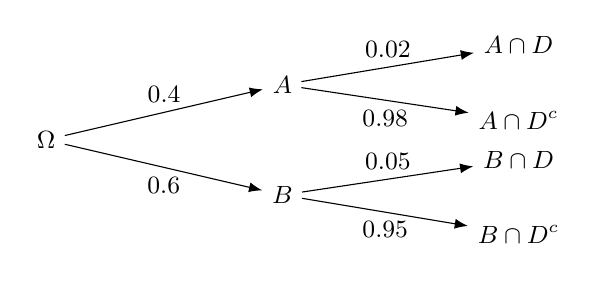
\begin{tikzpicture}[font=\small,>=Latex,line cap=round,line join=round]

\node (o) at (0,0) {$\Omega$};
\node (a) at (3,.7) {$A$}; \node (b) at (3,-.7) {$B$};
\node (ad) at (6,1.2) {$A\cap D$}; \node (ac) at (6,.25) {$A\cap D^c$};
\node (bd) at (6,-.25) {$B\cap D$}; \node (bc) at (6,-1.2) {$B\cap D^c$};
\draw[->] (o)--node[above]{$0.4$}(a); \draw[->] (o)--node[below]{$0.6$}(b);
\draw[->] (a)--node[above]{$0.02$}(ad); \draw[->] (a)--node[below]{$0.98$}(ac);
\draw[->] (b)--node[above]{$0.05$}(bd); \draw[->] (b)--node[below]{$0.95$}(bc);
\end{tikzpicture}
\end{document}
